
\begin{figure}[H]
\centering
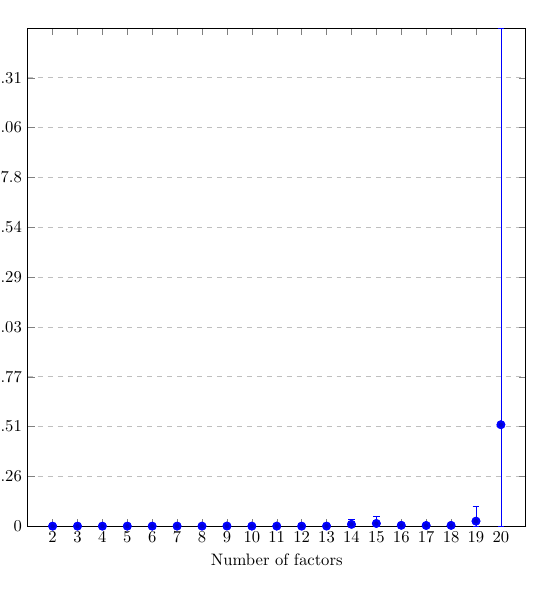
\begin{tikzpicture}[scale=0.6, trim axis left, trim axis right]
\begin{axis}[
    width=1\textwidth,
    height=1\textwidth,
    xlabel={Number of factors},
    ylabel={Time taken (s)},
    xmin=1.0, xmax=21.0,
    ymin=8e-06, ymax=182.571152,
    xticklabels={2, 3, 4, 5, 6, 7, 8, 9, 10, 11, 12, 13, 14, 15, 16, 17, 18, 19, 20},
    xtick={2, 3, 4, 5, 6, 7, 8, 9, 10, 11, 12, 13, 14, 15, 16, 17, 18, 19, 20},
    ytick={8e-06, 18.2571224, 36.5142368, 54.7713512, 73.0284656, 91.28558, 109.5426944, 127.7998088, 146.0569232, 164.3140376},
    ymajorgrids=true,
    grid style=dashed,
]

\addplot+[
    blue,
    very thick,
    forget plot,
    only marks
    ]
    plot[
    very thick,
    error bars/.cd,
    y dir=plus,
    y explicit
    ]
    table[x=x,y=y,y error expr=\thisrow{y-max}] {
    x    y    y-max
    11	0.007222025	0.007654975
10	0.00444145	0.00517855
13	0.018719475	0.015352525
12	0.0053848375	0.0140911625
20	37.1753798641	145.395772136
14	0.6586703125	1.8850956875
17	0.24851315	0.41537585
16	0.3026566625	0.5351573375
19	1.821185375	5.394434625
18	0.2796638	0.5461852
15	0.981518775	2.538424225
3	0.000693825	0.000648175
2	1.28e-05	2.22e-05
5	0.006653375	0.012691625
4	5.4075e-05	3.0925e-05
7	0.01022545	0.02771755
6	0.002554575	0.007333425
9	0.0283259	0.0499241
8	0.0008245625	0.0009594375

    };

\addplot+[
    blue,
    very thick,
    forget plot,
    only marks
    ]
    plot[
    very thick,
    error bars/.cd,
    y dir=plus,
    y explicit
    ]
    table[x=x,y=y,y error expr=\thisrow{y-min}] {
    x    y    y-min
    11	0.007222025	-0.007030025
10	0.00444145	-0.00400445
13	0.018719475	-0.018220475
12	0.0053848375	-0.0044008375
20	37.1753798641	-37.1712888641
14	0.6586703125	-0.6551153125
17	0.24851315	-0.24310915
16	0.3026566625	-0.3012356625
19	1.821185375	-1.794911375
18	0.2796638	-0.2752278
15	0.981518775	-0.976705775
3	0.000693825	-0.000625825
2	1.28e-05	-4.8e-06
5	0.006653375	-0.006581375
4	5.4075e-05	-1.1075e-05
7	0.01022545	-0.01001545
6	0.002554575	-0.002439575
9	0.0283259	-0.0280909
8	0.0008245625	-0.0005235625

    };

\end{axis}
\end{tikzpicture}
\vspace{-0.3cm}
\caption{Small primes, close primes}\label{fig:FermatsFactorizationSmallclose}
\end{figure}
